\section{Uppgift 2}\label{sec:uppg02}

\subsection{Instruktioner}
\begin{verbatim}
2. Skriv en klass FlygPlan som representerar ett flygplan. Klassens
   instansvariabler är:

   * höjd (int)
   * flygriktning (int)
   * hastighet (int)
   * modellbeteckning (String)

   Lämplig datatyp står inom parentes. När det gäller instansvariabeln
   flygriktning så ska den ha värdet 0 om planet står stilla, värdet 1 vid
   nordlig riktning, 2 ostlig, 3 sydlig och 4 västlig.

   Metoder ska finnas för följande operationer:

   - ändra planets höjd
   - returnera planets höjd
   - ändra planets flygriktning
   - returnera planets flygriktning
   - ändra planets hastighet
   - returnera planets hastighet
   - ändra planets modellbeteckning
   - returnera planets modellbeteckning
   - skriv ut alla data om flygplanet, metoden ska ha returtypen void

   Glöm ej konstruktorn.

   Skriv sedan ett testprogram som testar klassens metoder. Skapa minst 2
   stycken FlygPlans-objekt och testa metoderna på dessa objekt.
\end{verbatim}


\subsection{Kommentar}
Jag har valt att använda datatypen \texttt{enum} för att lösa uppgiften.  I
instruktionerna efterfrågas numeriska värden för flygriktningen och min lösning
uppfyller det kravet genom att metoden \texttt{getordinal()} från typen
\texttt{enum} används för att hämta de implicita värden som tillskrivs de olika
flygriktningarna i \texttt{Flygriktning} efter den ordningen de deklareras.
Min lösning för att "sätta" värdet hos en variabel av tyen
\texttt{Flygriktning} med en \texttt{int} är bristfällig, en mer sofistikerad
lösning skulle kunna använda mer avancerade funktioner hos typen \texttt{enum}.
Användandet av \texttt{enum} baseras på information från
\mbox{The Java Tutorials -- Enum Types}.
\footnote{\url{https://docs.oracle.com/javase/tutorial/java/javaOO/enum.html}}


\subsection{Källkod}
\javacode{src/Lab3Uppg02/Flygriktning.java}
\caption{Flygriktning.java}
\label{src:flygriktning}

\subsection{Källkod}
\javacode{src/Lab3Uppg02/FlygPlan.java}
\caption{FlygPlan.java}
\label{src:flygplan}

\subsection{Källkod}
\javacode{src/Lab3Uppg02/Lab3Uppg02.java}
\caption{Lab3Uppg02.java}
\label{src:uppg02}


\subsection{Skärmdump}
\begin{figure}[htbp]
    \centering
        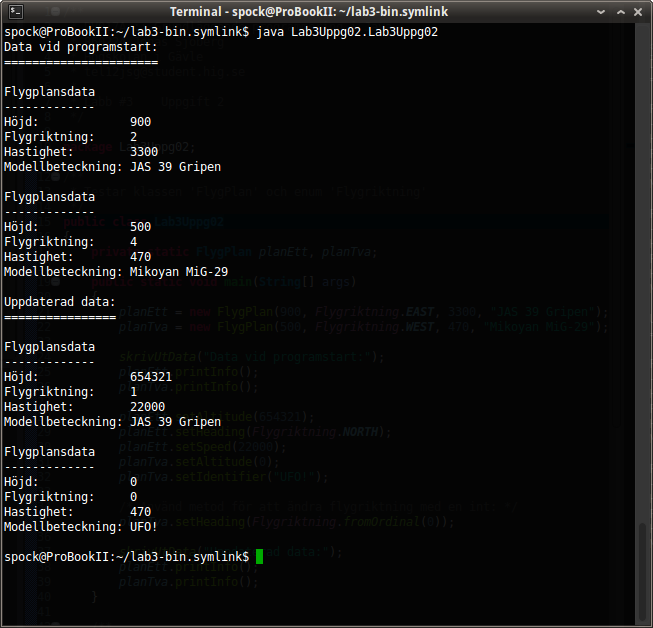
\includegraphics[width=\linewidth]{img/02.png}
    \caption{Körning av koden till Uppgift~\ref{sec:uppg02}}
    \label{fig:uppg02-screenshot}
\end{figure}

